\documentclass[a4paper, 12pt]{article}
\usepackage[left=2cm,right=2cm]{geometry}
\usepackage{times}
\usepackage[numbers]{natbib}
\usepackage[french]{babel}
\usepackage[utf8]{inputenc}
\usepackage[T1]{fontenc}
\usepackage{xcolor}
\usepackage{hyperref}

% listings support
\usepackage{listings}
\usepackage{verbatim}
\lstset{
  language=Java,
  extendedchars=true,
  inputencoding=utf8,
  basicstyle=\ttfamily,
  literate=
    {à}{{\`a}}1 {â}{{\^a}}1 {ç}{{\c{c}}}1 {é}{{\'e}}1 {è}{{\`e}}1
    {ê}{{\^e}}1 {ë}{{\"e}}1 {î}{{\^i}}1 {ï}{{\"i}}1 {ô}{{\^o}}1
    {û}{{\^u}}1 {ü}{{\"u}}1 {Ç}{{\c{C}}}1 {É}{{\'E}}1 {È}{{\`E}}1
    {Ê}{{\^E}}1 {Ë}{{\"E}}1 {Î}{{\^I}}1 {Ï}{{\"I}}1 {Ô}{{\^O}}1
    {Û}{{\^U}}1 {Ü}{{\"U}}1,
}

% to make nice graph figures
\usepackage{tikz}
\usetikzlibrary{shapes,arrows}
\usetikzlibrary{arrows.meta}

% formatting specifics
\setlength{\parindent}{0pt} % sets default to \noindent
% use \hspace{1em} for indentation
\usepackage{multicol}

% basic math package
\usepackage{amssymb}
\usepackage{amsmath}

% bibliography
\usepackage[numbib, nottoc]{tocbibind}
\bibliographystyle{plainnat}
\newcommand{\figref}[1]{(fig.\ref{#1}, p.\pageref{#1})}

% for figures and images
\usepackage{float}
\usepackage{graphicx}
\usepackage{graphbox}
\usepackage{subfig} %use subcaption for better compatibility

\title{Projet de Traitement de Signal et Télécommunications \\
\Large Étude d’une chaine de transmission sur porteuse pour une transmission
satellite fixe}
\author{Nicolas BAILLIET \and Paul LOUKA}
\date{\today}

\begin{document}
\maketitle
\tableofcontents

\clearpage
\section{Implantation d'une transmission avec transposition de fréquence}

\subsection{}

\begin{figure}[H]
    \centering
    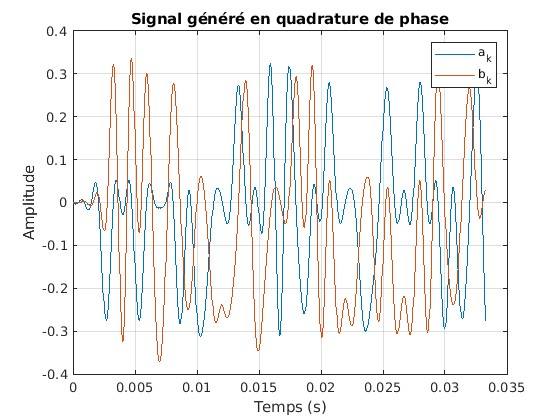
\includegraphics[width=0.5\textwidth]{graphics/1-1.jpg}
    \caption{Signaux générés sur les voies en phases et en quadrature}
    \label{fig:mon_etiquette}
\end{figure}

\subsection{}
\begin{figure}[H]
    \centering
    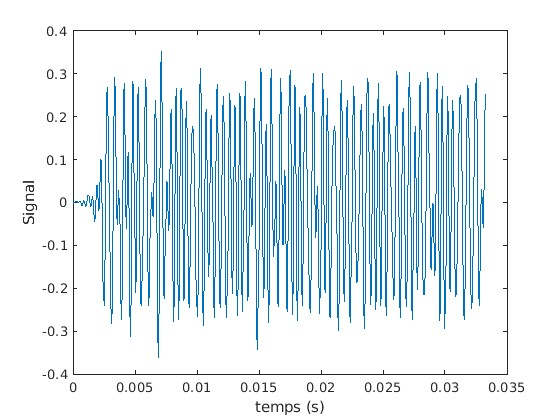
\includegraphics[width=0.5\textwidth]{graphics/1-2.jpg}
    \caption{Signal transmis sur fréquence porteuse}
    \label{fig:mon_etiquette}
\end{figure}

\subsection{}

\begin{figure}[H]
    \centering
    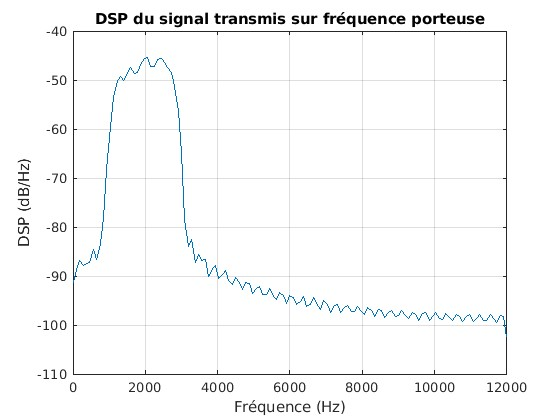
\includegraphics[width=0.5\textwidth]{graphics/1-3.jpg}
    \caption{DSP du signal transmis sur fréquence porteuse} 
    \label{fig:mon_etiquette}
\end{figure}

\subsection{}

\subsection{}

\begin{figure}[H]
    \centering
    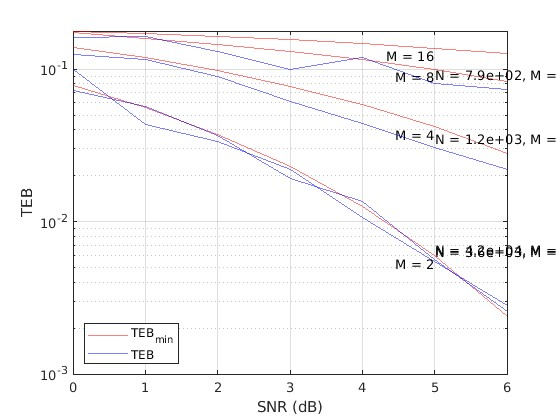
\includegraphics[width=0.5\textwidth]{graphics/1-5.jpg}
    \caption{TEB en fonction du SNR par bit à l'entrée du récepteur}
    \label{fig:mon_etiquette}
\end{figure}

\subsection{}

\clearpage
\section{Implantation de la chaine passe-bas équivalente à la chaine de transmission sur porteuse précédente}

\subsection{}
\begin{figure}[H]
    \centering
    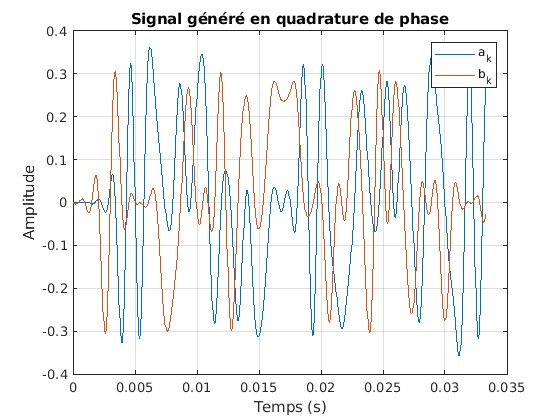
\includegraphics[width=0.5\textwidth]{graphics/2-1.jpg}
    \caption{Signaux générés sur les voies en phases et en quadrature}
    \label{fig:mon_etiquette}
\end{figure}

\subsection{}
\begin{figure}[H]
    \centering
    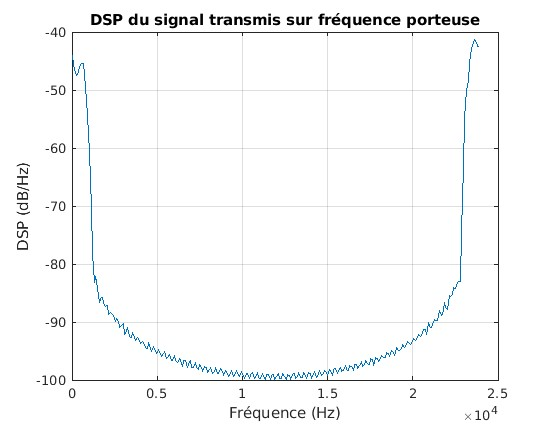
\includegraphics[width=0.5\textwidth]{graphics/2-2.jpg}
    \caption{DSP associée au signal transmis sur fréquence porteuse}
    \label{fig:mon_etiquette}
\end{figure}

\subsection{}

\subsection{}
\begin{figure}[H]
    \centering
    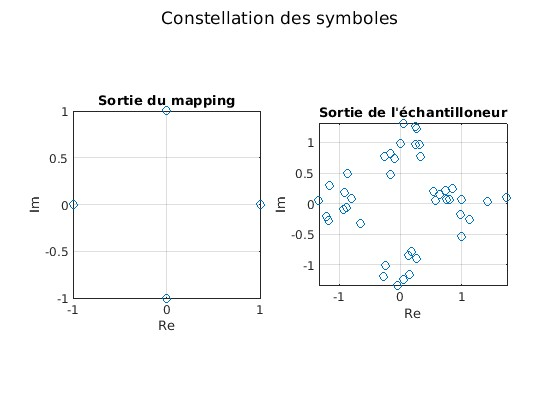
\includegraphics[width=0.5\textwidth]{graphics/2-4.jpg}
    \caption{Constellation en sortie de mapping}
    \label{fig:mon_etiquette}
\end{figure}


\subsection{}
\begin{figure}[H]
    \centering
    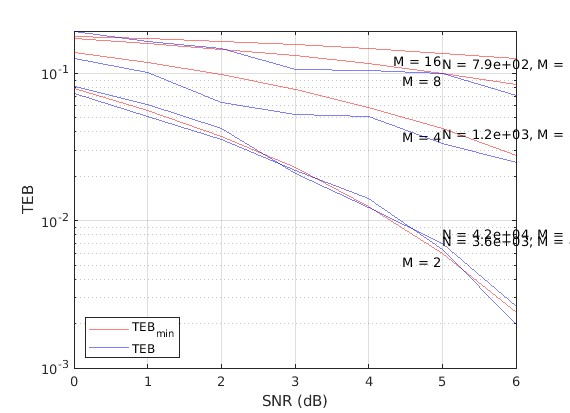
\includegraphics[width=0.5\textwidth]{graphics/2-5.jpg}
    \caption{TEB en fonction du SNR par bit à l'entrée du récepteur}
    \label{fig:mon_etiquette}
\end{figure}

\subsection{}

\clearpage
\section{Comparaison du modulateur DVS-S avec un des modulateur proposés par le DVB-S2}



\clearpage
\appendix
\section{APPENDIX}


\end{document}
